\documentclass[letterpaper,10pt]{article}
\usepackage{graphicx}
\usepackage{verbatim}
\usepackage{epsfig}

% \usepackage{}

\title{The MOOS-IvP Build System}
\author{Christian Convey (christian.convey@navy.mil)}
\date{2007-08-14}

\begin{document}

\maketitle

\begin{abstract}
This document details the design and intended use of MOOS-IvP's build system.
\end{abstract}

\tableofcontents

\parskip 7.2pt           % sets spacing between paragraphs

\section{HOWTO Build MOOS-IvP}
This section gives some basic background in using any CMake-based build system,
and then explains how to use MOOS-IvP's particular build system.

\subsection{CMake}

\subsubsection{Overview}
This section gives a brief overview of CMake, but clearer and more complete sources
of information exist:
\begin{itemize}
 \item The project's website: \verb|cmake.org|
 \item \underline{Mastering CMake}, by Ken Martin and Bill Hoffman.
 \item The CMake users email list: \verb|cmake@cmake.org|.  You can sign up
   for this at the \verb|cmake.org| website.
\end{itemize}


CMake (\verb|cmake.org|) is a cross-platform build system.  Compared to traditional 
Makefiles, CMake's control files (named \verb|CMakeLists.txt|) tend to be much shorter
and easier to read.

CMake has a number of back-ends for various operating systems and Make programs
(gmake, nmake, etc.) and IDEs (MS VisualStudio, KDevelop, Apple's XCode, etc.)
CMake-based build systems trivially support some features that can be a real
hassle to implement in hand-written Makefiles, such as calculating header file
dependencies and supporting an \verb|install| target.

The \verb|cmake| program reads in a project's \verb|CMakeLists.txt| files and produces
one or more files suitable for use in your build-system of choice (GNU Make, 
MS VisualStudio, etc.)  These generated build files will typically invoke the
\verb|cmake| program when building certain targets; therefore CMake must be installed
on any computer that will execute \verb|cmake|-produced build files.

\subsubsection{Language for Describing Makefiles}
\verb|CMakeLists.txt| files are written in an imperative language which is
documented on CMake's website.  The language lets you set variables and
supports branching, looping, and a limited form of subroutines (called
\verb|MACRO|'s).

When \verb|cmake| processes a project's \verb|CMakeLists.txt| files, the program
embodied in those files specifies the details of the build system to be created.
The \verb|CMakeLists.txt| files execute sequentially, specifying details as they
run.  Then end product is not a fully built version of your project, but rather
a set of build files (\verb|Makefile|, etc.) that when executed will build your
project.

The sequential nature of the programming language lets variables be computed,
helper programs run, conditions to be tested, etc. in order to determine what should
happen when the person building the project finally runs \verb|make| (or performs the
equivalent action in VisualStudio, XCode, etc. ).

\subsubsection{Federated Builds}
A typical CMake-based build system will contain one \verb|CMakeLists.txt| file
in each of the project's source tree's directories.  A simplified depiction
of this scheme is shown in Figure \ref{fig:cmake-file-tree}.


\begin{figure}
 \centering
\includegraphics[width=4in]{cmake-file-tree.eps}
   \caption{Conventionally each directory in the source code tree contains a CMakeLists.txt file.}
   \label{fig:cmake-file-tree}
\end{figure}


The project's \textit{top-level} \verb|CMakeLists.txt| file typically sets variables that
govern the entire project's build details, such as the directory into which 
the built libraries and / or executables should be placed after being linked, and
the directory(ies) in which the project's header files can be found.

The \verb|CMakeLists.txt| files
in the \textit{internal levels} of the source tree often do nothing other than call
\verb|ADD_SUBDIRECTORY| on each of that directory's subdirectories.
(\verb|ADD_SUBDIRECTORY| is very
similar in effect to the C preprocessor's \verb|#include| directive.)
The practice of having intermediate-level directories' \verb|CMakeLists.txt|
files mostly just consist of \verb|ADD_SUBDIRECTORY| is common because
those directories often exist merely to group together 
subdirectories into units that are meaningful to the programmer.
Therefore those directories have little significance to the way the 
project code is actually built.

The source tree's \textit{leaf directories} typically contain the bulk of the project's 
interesting source code, with each subdirectory having the code for a single
library or executable.  The \verb|CMakeLists.txt| file in one of these leaf
directories will generally contain an \verb|ADD_LIBRARY| or \verb|ADD_EXECUTABLE|
command which leads to the compilation and linking of that one particular
program / library.

\subsubsection{Inherited Variables}
\verb|CMakeLists.txt| scripts have variables, similar in form and purpose
to \verb|make| shell variables.  They're treated and manipulated as text, and
lists are generally represented as a single string in which spaces separate
the list's elements.  (Another convention is sometimes used in CMake's functions,
where semicolons rather than spaces separate list elements.)

In traditional \verb|Makefile|s, a child \verb|make| process inherits a 
parent \verb|make| process' variable values.  A similar effect exists in
a hierarchy of \verb|CMakeLists.txt| files, but via a different mechanism:

Consider Figure \ref{fig:cmake-file-structure}.  Using these 
\verb|CMakeLists.txt| files would look like this:
\begin{verbatim}
cmake -f CMakeLists.txt
(... some miscellaneous output from cmake ...)
Y
X
(... some miscellaneous output from cmake ...)
\end{verbatim} 

Notice how the subdirectory's file \verb|Bar/CMakeLists.txt| not 
only inherits a value of \verb|MyVar| from the parent \verb|CMakeLists.txt| 
file, but \verb|Bar/CMakeLists.txt| also affects the behavior of the
parent \verb|CMakeLists.txt| file.  (\verb|Bar/CMakeLists.txt|) modifies
the value of \verb|MyVar|, and that new value is in effect in the 
lines of the parent \verb|CMakeLists.txt| file that follow the 
\verb|ADD_SUBDIRECTORY| call.  

Contrast this to behavior to a \verb|Makefile|-based system where 
a parent directory's \verb|Makefile| calls \verb|make -f Bar/Makefile|.
In that scenario, there is no mechanism by which \verb|Bar/Makefile|'s
modifications of \verb|make| variables could propagate back to the 
parent directory's running instance of \verb|make|.

\begin{figure}
 \centering
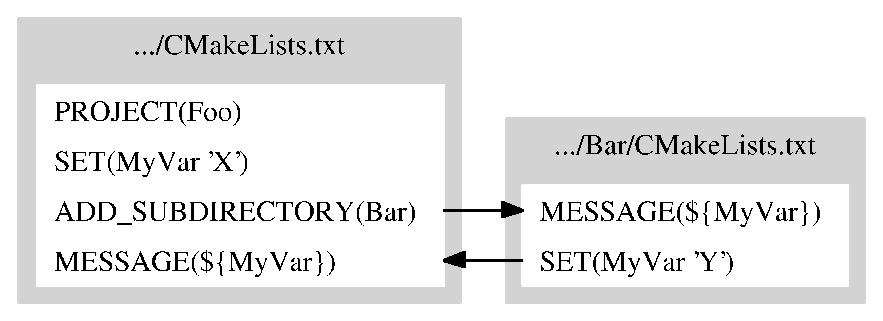
\includegraphics[width=4in]{file-structure.eps}
   \caption{ADD\_SUBDIRECTORY joins CMakeLists.txt files much like C's include}
   \label{fig:cmake-file-structure}
\end{figure}

\subsubsection{Cache Files}
Some CMake variables are computed each time you run \verb|cmake|, but other
\textit{cached} variables, once set, have their values recorded and stored in
a file named \verb|CMakeCache.txt|.  Variables stored in this file can be
edited using the \verb|ccmake| program (Linux) or the \verb|CMakeSetup.exe|
program (Windows).  This not only lets users enter certain data just one time
(i.e., the string that specifies the version of MOOS being built), but it also
exposes some CMake variables that whose value the user might want to correct.

For example, when CMake looks for the FLTK libraries, one variable that gets
set is \verb|FLTK_DIR|.  If CMake's \verb|FindFLTK| package can't figure out
where the FLTK libraries are, it will set the cached \verb|FLTK_DIR| variable
to have a value of \verb|FLTK_DIR-NOTFOUND|.  The user can run \verb|ccmake|
or \verb|CMakeSetup.exe| to manually set the value of \verb|FLTK_DIR| to
a valid value (typically \verb|/usr/lib| for that particular variable), and
then re-run \verb|cmake|.  This is typically enough of a help for a CMake
package such as \verb|FindFLTK| package to work out the rest of the details it
needs to.

Sometimes a \verb|CMakeCache.txt| file will contain so many bad values that
the user decides it's better just to start from scratch.  In general it's
safe for a user to manually delete a \verb|CMakeCache.txt| file.  When he
next runs \verb|cmake|, the variables whose values had been contained in the
file will simply be freshly computed.

\subsubsection{cmake, ccmake, CMakeSetup.exe}
\label{sec:ccmake}
Figure \ref{fig:cmake-data-flow} shows the relationship between CMake, the traditional
\verb|make| program, and various control files.
\verb|cmake| is used to generate build-system files from a set of \verb|CMakeLists.txt|
files.  \verb|cmake| will also read from and write to a \verb|CMakeCache.txt| in the
directory from which \verb|cmake| is run.


\begin{figure}
 \centering
\includegraphics[width=4in]{cmake-data-flow.eps}
   \caption{Build-time relationship between CMake, make, and their control files}
   \label{fig:cmake-data-flow}
\end{figure}



Sometimes \verb|cmake| doesn't succeed the first time it's run.  The FLTK module from
above is a good example.  We can easily write \verb|CMakeLists.txt| that would terminate
the \verb|cmake| invocation if the cached \verb|FLTK_DIR| variable had a value of \verb|FLTK_DIR-NOTFOUND|.

One solution to such a problem would be for the user to specify a good value on the
\verb|cmake| command line.  For example:
\begin{verbatim}
> cmake -DFLTK_DIR=/usr/lib -f CMakeLists.txt
\end{verbatim} 

This approach is sometimes the best, but \verb|ccmake| and \verb|CMakeSetup.exe| offer a
more interactive approach to configuring the build system.  Within these tools, you continue
re-running \verb|cmake| and modifing cached variable values until the \verb|cmake| succeeds.
At that point the user instructs the tool to ``generate'' the build system files (on Linux,
this typically includes a set of \verb|Makefile|s).  Once this is done the user will 
be ready to run \verb|make| (or whatever the equivalent action is for his build tool).

Note that \verb|ccmake| and \verb|CMakeSetup.exe| will not create the build system files
until the set of CMake variable values has stabilized.  This means that the tool must observe
that when it runs \verb|cmake|, none of the cached variables' values have changed.  This
relates to the fact that run \textit{n} of \verb|cmake| may set new value in a cached variable,
but the ramifications of that new variable aren't fully realized until the next invocation of
\verb|cmake| makes use of that value.

Practically speaking the need to iteratively run \verb|cmake| within \verb|ccmake| and \verb|CMakeSetup.exe| doesn't feel burdensome.  And if one knows the proper values for all
of the CMake variables of interest, you can set them on the \verb|cmake| command line 
as shown above, thus entirely avoiding the need to run \verb|ccmake| or
\verb|CMakeSetup.exe|.

\subsubsection{Finding External Packages}
When it comes to telling the build system where to find the header files and
development libraries for external packages such as FLTK or libGLU, CMake is
similar to GNU's \verb|autoconf|:  Contributors write CMake modules to discover 
the details needed to use a particular program, library, etc.  \verb|automake|
packages are written in the \verb|m4| macro language, whereas CMake modules are
written in CMake's scripting language - the same language used in 
\verb|CMakeLists.txt| files.  

CMake includes a number of these packages as a 
part of its standard distribution.  On Ubuntu Linux you can see those modules
in the directory 

\begin{verbatim}
 /usr/share/cmake-2.4/Modules/
\end{verbatim} 


You can also write your
own modules, but you need to tell CMake about which directories to search when
looking for extra modules that you've written.

Sometimes the standard supplied modules are of lower quality and you might want
to use your own CMake code instead.  A good example is \verb|FindFLTK|, 
which is used by both MOOS and IvP in order to discover the locations of the
include files and libraries for the FLTK library.  \verb|FindFLTK| does a bad
job of discovering the locations of these files, even if they're in
\verb|/usr/include/FL| and \verb|/usr/lib|, as expected.  \verb|FindFLTK| is 
also structured so that it's inconvenient to test whether or not FLTKs header
files and libraries have been found, without also requireding that the 
\verb|fluid| program (unused by MOOS and IvP) is installed.

MOOS avoids this quality problem by using a customized version of the module,
implemented in the file:

\verb|MOOS/MOOSFindFLTK.cmake|

But even that customized version of \verb|FindFLTK| has a painfully complex
implementation, and it still needs help just to realize that it should look
in the directory \verb|/usr/lib|
to find the FLTK libraries.


\subsubsection{Multiple Attempts to Configure the Project}
\textit{Configuring} a CMake-based project is the act of attempting to create
the build files (i.e., \verb|Makefile|, etc.) needed to build your software.
As described in Section \ref{sec:ccmake}, this make require multiple attempts
in order to ensure that all of the important CMake variables have the values
required to build your software the way you want it.

\subsubsection{In-source vs. Out-of-source Builds}
Sometimes we want to maintain multiple builds of the same software, where the builds
differ by details such as debug vs. optimized build, or perhaps where files will be
copied to if one were to run the command \verb|make install|.  (In the MOOS-IvP
project, the scripts for creating the Debian package files rely on this feature.)

To support the concurrent existence of multiple kinds of builds, the binaries
produced by the build process (object files, libraries, and programs) for different
types of builds must reside in different directories.  Even the generated Makefiles
for the different build types must be separated, because (for example) the directories
to which files will be copied when \verb|make install| is run are stored in the
Makefiles generated by CMake.

An \textit{in-source build} is one where the Makefiles, object files, etc. associated 
with a build of the software are stored in the same directory tree as the source files 
themselves.  An \textit{out-of-source build} is one where the Makefiles generated by
CMake, and the object files, libraries, and programs produced by those Makefiles, are
stored in a different directory tree than that in which the source code resides.

CMake can accomodate either in-source or out-of-source builds.  
When one creates an out-of-source build, CMake will generally create a
directory tree whose structure mirrors that of the source tree, and populate that 
newly created directory tree with Makefiles and various extra subdirectories needed
to fully build the software.  When one creates an in-source build, CMake will place
those same Makefiles and extra subdirectories directly into the appropriate locations
within the source code's directory tree.

When one runs \verb|cmake| or \verb|ccmake| or \verb|CMakeSetup.exe| to initially
configure a project, he passes as a command-line argument the root of the source 
code directory tree.  CMake will look within that specified directory tree for
the \verb|CMakeLists.txt| files that guide the creation of the build files, but
it will create the build files (\verb|Makefile|, etc.) in the current working 
directory from which \verb|cmake| was invoked.  Therefore an in-source build
tends to look like this:
\begin{verbatim}
cd ~/MyProj/src
ccmake ./
make
\end{verbatim} 

and an out-of-source build tends to look liks this:
\begin{verbatim}
mkdir ~/MyBuildDir
cd ~/MyBuildDir
ccmake ~/MyProj/src
make
\end{verbatim} 


It's often preferable to use out-of-source builds when possible.  When one
configures a project using \verb|cmake| (or \verb|ccmake| or 
\verb|CMakeSetup.exe|), certain details become fixed and cannot be changed
no matter what environment variables you set prior to running \verb|make|
within that build tree.  Examples include whether the code will be built
in debug or release mode (governed by the value of the \verb|CMAKE_BUILD_TYPE|
variable), and where files will be installed if you run \verb|make install|
(governed by the value of the \verb|CMAKE_INSTALL_PREFIX| variable).  

If one wants to rapidly switch, for example, between release and debug builds,
then it may be desirable to maintain two separate out-of-source configurations
that differ only in their value of the \verb|CMAKE_BUILD_TYPE| variable.  One
might therefore do something like this:

\begin{verbatim}
mkdir ~/MyBuildDir/release
~/MyBuildDir/release
ccmake -DCMAKE_BUILD_TYPE=Release ~/MyProj/src
make

mkdir ~/MyBuildDir/debug
~/MyBuildDir/debug
ccmake -DCMAKE_BUILD_TYPE=Debug ~/MyProj/src
make
\end{verbatim} 


Another example of where the use of out-of-source configurations is useful 
is when the MOOS-IvP build system produces Debian packages.  Our technique
for producing the different Debian packages involves varying the value of
the \verb|CMAKE_INSTALL_COMPONENT| CMake variable.  It seemed overly intrusive
to re-configure the build directory used by the person creating the Debian
packages, so the Debian packaging scripts use out-of-source builds whose
configurations have various values for the \verb|CMAKE_INSTALL_COMPONENT| 
CMake variable.

In order to remain consistent with the general behavior of the of IvP's
previous build system, the top level \verb|build.sh| script performs an
in-source build.  However, the MOOS-IvP project can be built equally well
as an out-of-source build.

\subsection{Source Tree Organization and the Two Build Systems}
When targeting a Make-based build system, \verb|cmake| will produce a set
of files named \verb|Makefile|, one in each directory of the tree.

In order to permit MOOS-IvP's old set of Makefiles to remain present in
the source tree, I renamed all of the old Makefiles to be named \verb|makefile|
(note the lower-case filename).  In the old make system, the makefile
in one directory builds the contents of its child directories by invoking
the command \verb|make -f (child-dir)/makefile|.  Because the tweaked version of the 
old build system specifically calls \verb|make| on the lower-case-named \verb|makefile|,
the two build systems manage to remain completely independent.

Our expectation is that after several months of gaining confidence in the CMake-based
build system, Mike Benjamin will permit the old \verb|makefile| files to be 
removed from the source tree.

\subsection{Building MOOS-IvP}

\subsubsection{Required Steps for old makefile-based build}
In contrast to a previous organization of the MOOS-IvP directory tree, the
\verb|ivp/src| no longer contains a subset of the programs and libraries that are
part of the MOOS project.  Therefore if one is using the old makefiles to build
IvP, he must first explicitly build the MOOS libraries so that they're available when
the ivp programs are being linked.  This is the primary difference between the old
and new technique for building IvP when using the old-style makefiles.

The steps are as follows:

\begin{enumerate}
 \item Check-out or download the moo-ivp source code, into some directory \verb|foo/|.
 \item Build MOOS:
 \begin{enumerate}
  \renewcommand{\labelenumii}{\arabic{enumi}.\arabic{enumii}.}
   \item \verb|cd foo/MOOS|
   \item \verb|../build.sh|

	If this step fails, you may need to modify one or more of the directories
	mentioned in the file \verb|../build.sh|.

	Note that MOOS is being built with CMake, even though these present instructions
	describe building IvP without using CMake.  This is because (a) we've decided to
	stop importing code from the MOOS project directly into the IvP source tree, and
	(b) the MOOS project uses CMake rather than hand-written makefiles.

 \end{enumerate}

 \item \verb|cd foo/ivp/src|
 \item \verb|make -f makefile|

	If you don't specify \verb|-f makefile|, and have previously used the
	CMake-based build system in this directory, then your invocation of \verb|make|
	will probable use the file \verb|ivp/src/Makefile| (note the upper-case \verb|M|).
	That file is created by CMake, which presumably isn't what you want since these
	present steps describe how to use IvP's \textit{non}-CMake build system.

\end{enumerate}


\subsubsection{Required Steps for CMake-based build (Easy Technique)}
\begin{enumerate}
 \item Check-out or download the moo-ivp source code, into some directory \verb|foo/|.
 \item \verb|cd foo/|
 \item \verb|./build.sh|
\end{enumerate}

\subsubsection{Required Steps for CMake-based build (Advanced Technique)}
This is the approach you'll need to take if CMake can't find some required header
file or library, or if you want to tweak what set of programs and libraries are
built.

\begin{enumerate}
 \item Check-out or download the moo-ivp source code, into some directory \verb|foo/|.
 \item \verb|cd foo/|
 \item \verb|ccmake -f CMakeLists.txt|

	Within \verb|ccmake|, set variables as desired until you can generate the
	build files.  Then generate them (within \verb|ccmake|).  Documentation of
	\verb|ccmake| and \verb|CMakeSetup.exe| is out of the scope of this document,
	but the book \underline{Mastering CMake} is an excellent source of information.
	An explanation can also be found here: 

	\verb|http://www.cmake.org/HTML/RunningCMake.html|

	Note that the file \verb|foo/build.sh| shows an invocation of \verb|cmake| that
	sets some CMake variables that the current build system has trouble figuring
	out on your own.  If you're having trouble getting any of those variables to
	take on good value when using \verb|ccmake|, consider using the respective
	values mentioned in \verb|foo/build.sh|

\item \verb|make|

\end{enumerate}


\subsubsection{Requried Ubuntu Packages}
The following is a (perhaps) partial list of packages that must be installed on a 
Ubuntu 7.04 (``Feisty Fawn'') system in order to build IvP and the non-Matlab parts
of MOOS:
\begin{center}
% use packages: array
\begin{tabular}{|l|l|}
\hline
Ubuntu package & Reason needed \\
\hline
\hline
mesa-common-dev & Requried to build programs that use FLTK + OpenGL \\
\hline
libfltk1.1-dev & Requried to build programs that use FLTK + OpenGL \\
\hline
libglu1-mesa-dev & Requried to build programs that use FLTK + OpenGL \\
\hline
libtiff4-dev & Requried to build programs that use FLTK + OpenGL \\
\hline
libxft & Requried to build programs that use FLTK + OpenGL \\
\hline
libxft-dev & Requried to build programs that use FLTK + OpenGL \\
\hline
fluid & To satisfy CMake's \verb|FindFLTK| module \\
\hline
cmake & Integral part of build system \\
\hline
python-dev & Required to build \verb|uVoice| (not built by default) \\
\hline
swig & Required to build \verb|uVoice| (not built by default) \\
\hline
\end{tabular}
\end{center}


\subsection{Important CMake Variables}
\subsubsection{For FLTK}
\begin{description}
 \item[FLTK\_DIR] - This is the library where CMake's \verb|FindFLTK| module expects to 
	find the FLTK libraries.  For mystifying reasons, it can't figure out on its own
	to look in \verb|/usr/lib|.  You will probably want to set this to \verb|/usr/lib|.

	As a bonus, once you do so, MOOS's customized version of that module, \verb|MOOSFindFLTK|,
	will be able to figure out the proper value for \verb|FLTK_INCLUDE_DIR| all by itself.
	As of this writing, IvP uses the standard version of \verb|FindFLTK| which sadly
	cannot figure out the proper value for \verb|FLTK_INCLUDE_DIR| after you've provided
	a valid value for \verb|FLTK_DIR|.

 \item[FLTK\_INCLUDE\_DIR] - The directory that is expected to include a subdirectory 
	named \verb|FL|,
	which in turn contains FLTK's source files.  On Ubuntu Linux 7.04, at least, the 
	proper value for this is \verb|/usr/include|.
 \end{description}

\subsubsection{For Python.h}
\begin{description}
 \item[IVP\_BUILD\_\_MOOS] - When this is \verb|ON| the build system will build \verb|uVoice|,
	a Python
	wrapper for MOOS's libraries.  When this is \verb|ON| you'll need to set a proper
	value for the CMake variable \verb|PYTHON_INCLUDE_PATH| or else the build processes
	won't attempt to build \verb|uVoice|.

 \item[PYTHON\_INCLUDE\_PATH] - The directory containing the version of \verb|Python.h| that
	should be used when building \verb|uVoice|.  On Ubuntu Linux 7.04, which by default
	uses Python version 2.5, the correct value for this variable is 
	\verb|/usr/include/python2.5|, assuming that you're trying to make a wrapper that
	works with the host system's version of Python.
 \end{description}

\subsubsection{Other CMake Variables}
\begin{description}
 \item[IVP\_BUILD\_...] - There's one of these variables for each program and library
	in the IvP part of the moos-ivp source tree.  Setting a value to \verb|ON| will
	cause the corresponding program or library to be included in the build process.

	Several programs / libraries that were by default \textit{not} built by the
	old build system have a default value of \verb|OFF| for this variable.  All others
	default to \verb|ON|.

	Note that the current IvP build system does not enforce, at this step, 
	the build dependencies between libraries and the programs that require them at
	link-time.  If you disabling the building of a library but enable the building
	of some program that must be linked to that library, you'll end up with an error
	from the linker when that program is being built.

 \item[BUILD\_...] - These come from the MOOS side of the project.  Setting one of these
	variables to \verb|ON| may lead to the appearance of even more such variables
	when you next configure the build tree, because MOOS's build system supports
	a two-level hierarchy of dis-/en-abling the building of its programs and libraries.

 \item[CMAKE\_BUILD\_TYPE] - By convention, any CMake variable whose name starts with
	\verb|CMAKE_| has special meaning to CMake.  This variable controls details related
	to debug vs. optimized builds.  Two noteworthy values are \verb|Debug| and \verb|Release|.

 \end{description}


\section{MOOS-IvP Build System Implementation Details}

\subsection{create-subdir-cmake-files.sh}
IvP's source tree contains about 79 libraries and applications as of this writing, each of
which requires its own \verb|CMakeLists.txt| file.  Most IvP programs have similar needs
for their \verb|CMakeLists.txt| files, and the same goes for most IvP libraries.

Because this regularity exists, and because all 79 of those \verb|CMakeLists.txt| files must
be rewritten when certain improvements are made to the build system, IvP contains a
script (plus a few helper files) to re-create those 79 \verb|CMakeLists.txt| files 
whenever required.

That script is named \verb|create-subdir-cmake-files.sh|.  It and its support files are 
found in the directory
\begin{verbatim}
ivp/scripts/util/create-subdir-cmake-files 
\end{verbatim} 

Whenever a library or program is added to or removed from IvP, this script should be
modified so that we can always easily recreate and / or redesign IvP's build system.

As of this writing, this script only creates IvP's \verb|CMakeLists.txt| files, and none
of MOOS's.  This is because the MOOS project already has a CMake-based build system in 
place and there's no obvious need to re-implement it.


\section{Future Work}


\subsection{Debian packaging}
Debian packaging can be accomplished by some minor additions to IvP's 
CMake-based build system.  We've already submitted a patch for doing this
in MOOS to Paul Newman, so the techniques and code have been worked out
already.

\subsection{RPM packaging}
CMake 2.6, expected to be released in late 2007, should have a feature for
easily producing RedHat Package Manager (RPM) software packages.  When this
happens we may support this for MOOS-IvP.

\subsection{Windows builds}
Now that all of MOOS-IvP can be built with CMake, we may be able to build
the software on Windows with little or no additional effort.

[Note: Andrew Shafer has protested that this may be an overly optimistic
assesment.]

\subsection{Windows packaging}
Develop an installation technique for MOOS-IvP that's convenient for Windows
programmers.  We haven't yet investigated what the most preferred form of
packaging is.

\subsection{Building Documentation}
CMake can easily build man pages, Doxygen documentation, etc.  Building it
with CMake helps us to package the documentation for end-user use, as well
as creating \verb|...-doc| Debian packages and whatever the RPM equivalent
would be.

\subsection{Building IvP's Website}
CMake's scripting language should be sufficient for expressing how to create
new versions of IvP's static html website.  This would be useful to ensure that
the website is always synchronized with the most current release of our software
and documentation.

\end{document}
